\chapter{Study Area}
Ob River (see figure \ref{fig:Ob Basin}), river of central Russia. One of the greatest rivers of Asia, the Ob flows north and west across western Siberia in a twisting diagonal from its sources in the Altai Mountains to its outlet through the Gulf of Ob into the Kara Sea of the Arctic Ocean. It is a major transportation artery, crossing territory at the heart of Russia that is extraordinarily varied in its physical environment and population. Even allowing for the barrenness of much of the region surrounding the lower course of the river and the ice-clogged waters into which it discharges, the Ob drains a region of great economic potential.\\\\
The Ob proper is formed by the junction of the Biya and Katun rivers, in the foothills of the Siberian sector of the Altai, from which it has a course of 2,268 miles (3,650 km). If, however, the Irtysh River is regarded as part of the main course rather than as the Ob's major tributary, the maximum length, from the source of the Black (Chorny) Irtysh in China's sector of the Altai, is 3,362 miles (5,410 km), making the Ob the seventh longest river in the world. The catchment area is approximately 1,150,000 square miles (2,975,000 square km). Constituting about half of the drainage basin of the Kara Sea, the Ob's catchment area is the sixth largest in the world.
\begin{figure}[htbp]
	\centering
	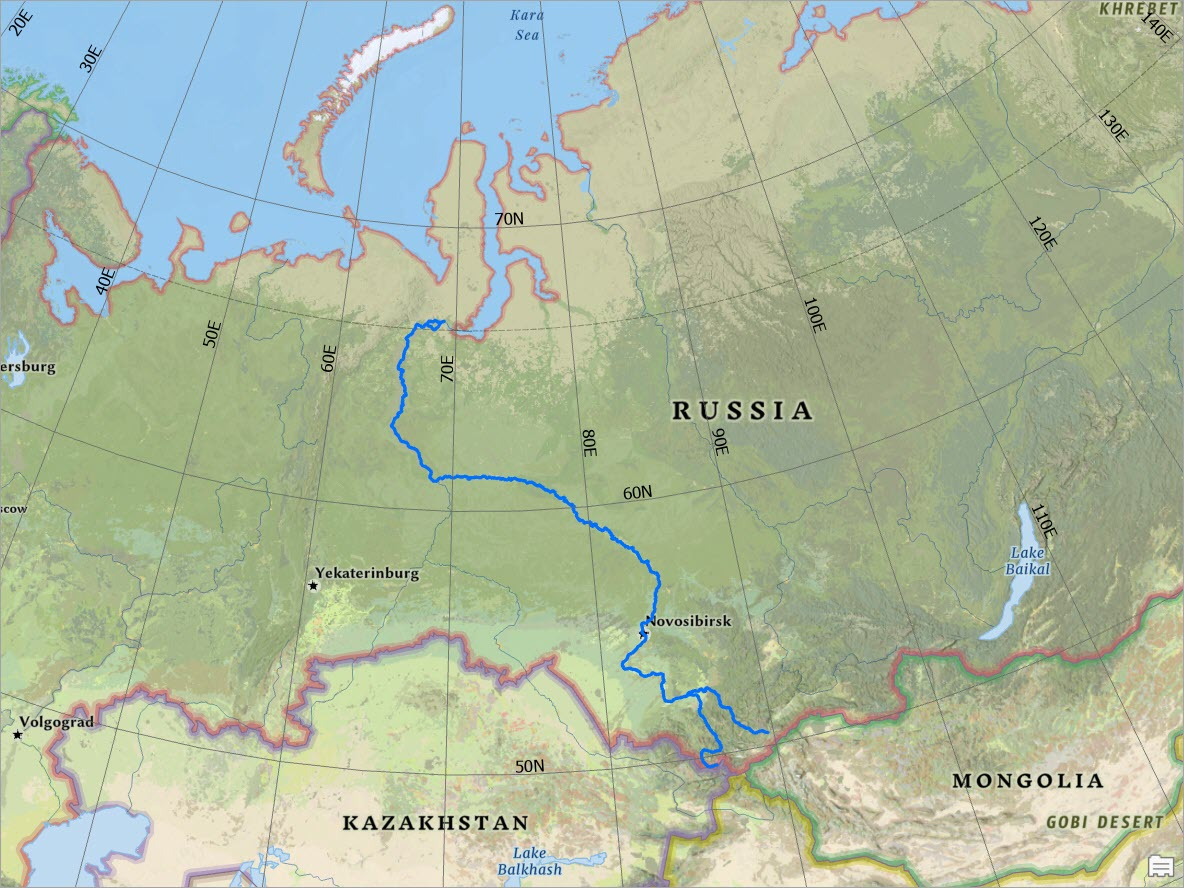
\includegraphics[width=0.7\textwidth]{river-basins-Ob-drainage-networks-Yenisey} % Datei in "bilder/" bei LaTeX: eps, bei PDFLaTeX: jpg (o.ä.) 
	\caption{River Basins Ob} 
	\label{fig:Ob Basin}
\end{figure}\\\\
The Ob basin has short, warm summers and long, cold winters. Average January temperatures range from  $-28 ^{\circ}$C on the shores of the Kara Sea to $-16 ^{\circ}$C in the upper reaches of the Irtysh. July temperatures for the same locations, respectively, range from 4 $^{\circ}$C to above $20 ^{\circ}$C. The absolute maximum temperature, in the arid south, is $40 ^{\circ}$C, and the minimum, in the Altai Mountains, is $-60 ^{\circ}$. Rainfall, which occurs mainly in the summer, averages less than 400 mm per year in the north, 500 to 600 mm in the taiga zone, and 300 to 400 mm on the steppes. The western slopes of the Altai receive as much as 1,575 mm per year. Snow cover lasts for 240 to 270 days in the north and for 160 to 170 days in the south. It is deepest in the forest zone, where it ranges from 60 to 90 cm, and in the mountains, where it averages 200 cm per year. It is much shallower on the tundra, ranging from 30 to 50 cm, and very thin on the steppe, where 20 to 40 cm fall.\\\\
The Ob River contributes on average 402 $\ut{km^3}$ freshwater per year, or about 15\% of total fresh water flow into the Arctic Ocean. The drainage basin is classified as cropland (36\%), forest (30\%), wetland (11\%), grassland (10\%), shrub (5\%) , developed (5\%) and irrigated cropland (3\%). Basin total population is about 27 million, with 39 cities having a population of more than 100 000. The steppe zones in the southern portion of the basin are the major wheat production regions in Russia. The west Siberian oil and gas field, located in the taiga and tundra zones of the middle and lower Ob, contribute about two-third of the country's crude oil and natural gas outputs.  